\documentclass[english,12pt,a4paper,titlepage]{article}
\usepackage{tgtermes}
\usepackage[T1]{fontenc}
\usepackage{newtxtext,newtxmath}
\usepackage[left=1in, right=1in, top=1in, bottom=1in]{geometry}
\usepackage{graphicx}
\usepackage{nameref}
\usepackage{babel}
\usepackage{etoolbox}
\usepackage{fancyhdr}
\usepackage{setspace}
\usepackage[citestyle=mla, style=mla-new]{biblatex}
\usepackage[hidelinks]{hyperref}
\usepackage{listings}
\usepackage[table]{xcolor}
\usepackage{booktabs}
\usepackage{siunitx}
\usepackage{adjustbox}
\usepackage{wrapfig}
\usepackage{float}
\usepackage{qrcode}

\addbibresource{references.bib}
\graphicspath{ {./res/} }

\AtBeginEnvironment{array}{\setlength{\arraycolsep}{25pt}}
\renewcommand{\arraystretch}{2}

\definecolor{codegreen}{rgb}{0,0.6,0}
\definecolor{codegray}{rgb}{0.5,0.5,0.5}
\definecolor{codepurple}{rgb}{0.58,0,0.82}
\definecolor{backcolour}{rgb}{0.95,0.95,0.92}

\raggedright
\setlength\parindent{24pt}

\lstdefinestyle{mystyle}{
	backgroundcolor=\color{backcolour},   
	commentstyle=\color{codegreen},
	keywordstyle=\color{magenta},
	numberstyle=\tiny\color{codegray},
	stringstyle=\color{codepurple},
	basicstyle=\ttfamily\tiny,
	breakatwhitespace=false,         
	breaklines=true,                 
	captionpos=b,                    
	keepspaces=true,                 
	numbers=left,                    
	numbersep=5pt,                  
	showspaces=false,                
	showstringspaces=false,
	showtabs=false,                  
	tabsize=1,
	linewidth=\textwidth,
	xleftmargin=-1.5cm,
	xrightmargin=-1.5cm
}

\lstset{style=mystyle}

\fancypagestyle{headerstyle}{
	\fancyhf{}
	\renewcommand{\headrulewidth}{0pt}
	\lhead[]{Emergency Situational Awareness \hspace*{\stretch{2}} Blaut \thepage\\}

}

\defbibheading{bibliography}[\bibname]{}

\begin{document}
	%/ Title Page
	\thispagestyle{empty}
	\vspace*{\stretch{3}}
	\label{Title Page}
	\begin{center}
		{\large\textbf{Enabling situational awareness during emergency events through inter-building nodes and a mobile application}}\\
		\[
		\begin{array}{cc}
			\mbox{Noah Blaut}\\
			\mbox{Hill Country Christian School of Austin}\\
			\mbox{March 6, 2026}
		\end{array}
		\]
		\vspace{1in}
		\[
		\begin{array}{cc}
			\mbox{\textbf{Thesis Teacher and Advisor}}\\
			\mbox{Hannah Sorley}\\
			\mbox{Carl Hannusch}
		\end{array}
		\]
	\end{center}
	\vspace*{\stretch{2}}
	
	\setcounter{page}{0}
	
	\newpage
	\pagestyle{headerstyle}
	\setstretch{2.0}
	\[
	\begin{array}{cc}
		\mbox{\bfseries{Abstract}}
		\label{Abstract}
	\end{array}
	\]
	
	The effective use of communication systems is critical for saving lives and coordinating first responders. As such, many emergencies require the rapid deployment of Emergency Communication Systems (ECS) capable of continuously transmitting, processing, and receiving data \autocite{Navarro}. These ECS devices come with high installation costs and are not easily accessible; they are crucial devices for first responders and other stakeholders, who need "as much in-field information as possible to forecast their strategy and operations” \autocite{Navarro}. Additionally, real-time, accurate information distribution during an emergency is a crucial component of improving outcomes during events. This device aims to address both of these issues by incorporating a two-part system of inter-room beacons and stakeholder mobile devices running a smartphone application capable of locating the device's position within a building and communicating emergency tasks and action items that can be adjusted by key personnel throughout the duration of an event, as recognized through an automated "playbook" system. Through testing and data analysis, this design has proven to meet all stakeholder needs and design considerations.
	
	\vspace*{1cm}
	\begin{minipage}{\textwidth}
		\centering
		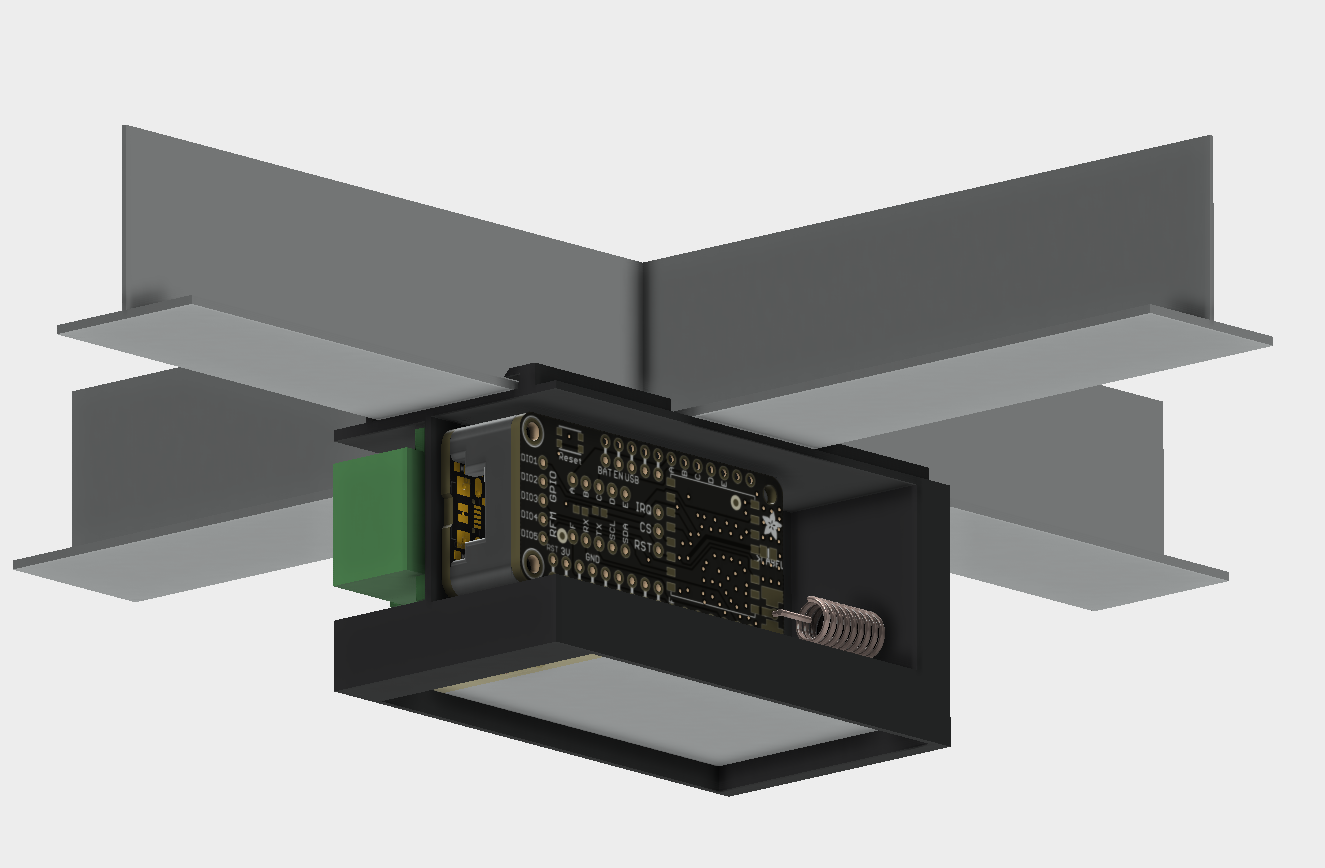
\includegraphics[width=.6\linewidth]{embody-1}
	\end{minipage}
	
	%/ Introduction
	\newpage
	\pagestyle{headerstyle}
	\setstretch{2.0}
	
	\[
	\begin{array}{cc}
		\mbox{\bfseries{Introduction}}
		\label{Introduction}
	\end{array}
	\]
	
	The past decade has brought major changes to emergency response planning, driven primarily by an increase in emergency incidents in the United States. Between the years of 2020 and 2024 and the previous five years, a 70\% increase in active shooter events was recorded in the United States \autocite{FBI2024}, leading to over 4,000 victims and more than 1,700 fatalities \autocite{Tucker2024}. In this quickly shifting landscape, more schools, churches, and businesses are creating emergency response plans to prepare for the worst.
	
	However, these disaster response and continuity-of-operations plans vary depending on the resources available in the environment in which they are being implemented. For example, in 2023, the nearby school district, Leander ISD, passed a bond package that budgeted over \$10 million for security improvements to its campuses, including \$330,000 for installing a crisis alert system \autocite{LeanderISDBond}. This system features a faculty panic alarm, upgrades and additions to lockdown buttons, the installation of visual strobe lights, and the creation of a “digital-twin” of building layouts for first responders to access through an online portal \autocite{LeanderISDBondSecurity}. However, not every school, church, or business can set aside such a large sum to fund security improvements, possibly leaving the people operating within these organizations at risk. Additionally, these panic alert systems, like those implemented by Leander ISD, come with high installation costs and increased overhead, and, as such, may dissuade organizations from investing. As a member of a school widely regarded by interviewed stakeholders as having an open campus, I believe that security improvements should not entail implementation costs so aggressive as to dissuade institutions from adopting potentially life-saving technology, and that existing solutions do not effectively meet the needs of widespread, distributed campus communities like our own.
	
	To address these issues, the development of this device followed various phases of the engineering design process to ensure it met all the identified needs of an emergency communications system. These phases included Identify, Describe, Generate, Select, and Embody.
	
	%/ Identify Phase
	\[
	\begin{array}{cc}
		\mbox{\bfseries{Identify Phase}}
		\label{Identify Phase}
	\end{array}
	\]
	
	The purpose of the Identify phase is to establish the growing need for communication systems that provide real-time insights into emergency situations across large, distributed campuses. During emergency situations, first responders rely on timely, accurate information to make informed life‑or‑death decisions under pressure. However, the flow of information in emergency situations can be hindered by the limitations of existing technologies. Issues such as limited implementation of technological solutions, damage to critical infrastructure, or communication channel failures all reduce the effectiveness of current solutions on the market. Addressing this gap requires identifying ways technology can enhance real-time communication and awareness, enabling faster, more effective responses.
	
	The effective use of communication systems is critical for saving lives and coordinating first responders. As such, many emergencies require the rapid deployment of Emergency Communication Systems (ECS) capable of continuously transmitting, processing, and receiving data \autocite{Navarro}. However, existing systems on the market today often fail to deliver high-quality, uninterrupted communication, with data transfer frequently occurring in simplex mode, where only one endpoint can send or receive data at a time \autocite{Navarro}. To effectively coordinate first responders and reduce the timeline of emergency events, first responders and other stakeholders “need as much in-field information as possible to forecast their strategy and operations” \autocite{Navarro}. With the guarantee of high-quality and reliable communications during an emergency, first responders and other stakeholders can respond most effectively to a variety of unknowns.
	
	Effective disaster response also depends on stakeholders having a comprehensive understanding of the situation they are entering into. According to Kedia et al., “Timely, accurate, and complete [situational awareness] is a key enabler of successful disaster response when the situation is changing rapidly, resources are limited, and different agencies must coordinate their activities.” \autocite{Kedia2022}. As such, an effective response requires rapid, accurate, and shared information across multiple agencies, while limitations in infrastructure, communications, data analysis, and interoperability can often undermine effective decision-making.
	
	This transmission of accurate, shared information occurs through systems such as the Internet of Emergency Services (IoES) frameworks, which provide real-time data collection and sharing, overcoming delays associated with more manual systems, such as radio endpoints. According to Damaševičius et al., “[IoES] technology can help automate and streamline emergency response processes . . .  providing real-time data and insights that can enable faster and more effective responses.” \autocite{Damasevicius2023}.
	
	By enhancing the efficiency of emergency response systems, the biblical values of protecting life and serving others are upheld. Genesis 1:27 and Psalm 139:13-14 show that “God created mankind in his own image,” \autocite{Genesis}, and each individual is “fearfully and wonderfully made.” \autocite{Psalm} As such, implementing technologies that improve communication and awareness in emergencies not only facilitates a more rapid response but also honors the image of God in every person, showing our responsibility to protect and serve as stewards of life.
	

	%/ Describe Phase
	\[
	\begin{array}{cc}
		\mbox{\bfseries{Describe Phase}}
		\label{Describe Phase}
	\end{array}
	\]
	
	Stakeholders in emergencies rely on multiple discrete data sources to transform information into effective insights and maintain awareness of an emergent event. While many solutions are available for aggregating these data sources, these systems usually rely on permanent building infrastructure, such as cameras, door sensors, and other networked devices, which require significant planning, installation, and annual maintenance costs. Additionally, such systems are vulnerable to instability caused by infrastructure disruptions during emergencies, including communication or power outages. This paper will examine existing approaches to maintaining situational awareness during emergencies, demonstrate the need for a solution independent of fixed infrastructure, and identify the requirements of key stakeholders involved in emergency response and management.
	
	\label{Describe Phase - Prior Solutions}
	\begin{flushleft}
		\bfseries{Existing Solutions}
	\end{flushleft}
	
	Emergency management technology has evolved rapidly with the introduction of Internet of Things (IoT) devices and advances in processing capabilities and software that enable connectivity with external devices and systems \autocite{Damasevicius2023}. This evolution has led to the development of a subset of IoT devices known as Internet of Emergency Services (IoES) devices. These devices can integrate with emergency service networks to enable informed emergency coordination based on real-time data insights \autocite{Damasevicius2023}. However, a common issue across both IoT and IoES systems is their reliance upon fixed infrastructure that can be compromised during crises, leaving those who rely on them in the dark and unable to access the mission-critical data needed to make effective decisions. 
	
	Over the past five years, emergency dispatch organizations have begun to adopt Integrated Emergency Data Platforms \autocite{Tantillo2025}. These systems integrate various data sources, customized to the area, to deliver actionable insights, advanced visualization, and comprehensive situational awareness to emergency communication centers.
	\begin{figure}[H]
		\setstretch{0.8}
		\centering
		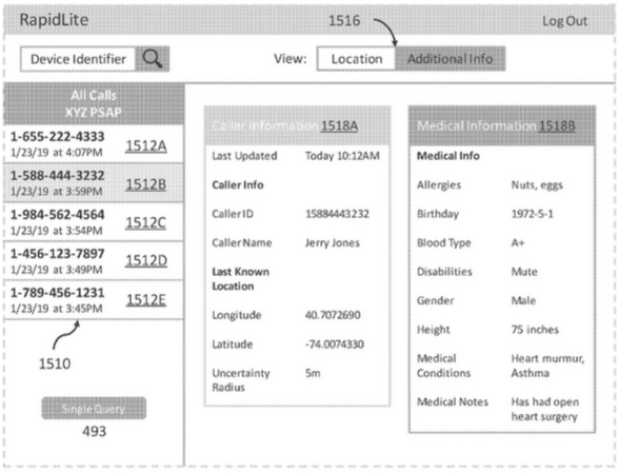
\includegraphics[width=.6\linewidth]{describe-1}
		\caption{US12432543B2 – Systems and User Interfaces for Emergency Data Integration}
		\label{fig:describe-1}
		\setstretch{2.0}
	\end{figure}
	Figure \ref{fig:describe-1} illustrates how these systems combine data from multiple sources, including Geographic Information System (GIS) datasets, phone registry records, and traffic sensor networks, and present the data in interactive graphical displays during emergencies \autocite{Pellegrini2025}. By allowing stakeholders unfamiliar with the environment to share floor plans, video feeds, and access controls, these systems can reduce emergency response times \autocite{Pellegrini2025}. However, the implementation of these platforms relies on pre-existing infrastructure, including stable network connections and building-embedded sensors, which can fail during power outages or physical damage. Combined with high installation costs and additional maintenance burdens, the scalability of these solutions is limited to large-scale facilities, which conflicts with stakeholder needs for low-dependency solutions that can operate inside dynamic environments. Additionally, stakeholders from a local emergency management division highlighted additional problems with these systems during interviews: the overwhelming volume of data makes it difficult to coordinate decision-making effectively, especially when emergencies require personnel to leave their command-and-control center workstations and respond in the field.
	
	The implementation of Integrated Emergency Data Platforms requires integrating many discrete data streams, often from connected sensors, IoT \& IoES devices, and video systems \autocite{Pellegrini2025}. Figure \ref{fig:describe-2} illustrates how the detection of a gunshot event can trigger an automated response plan via IoES sensor networks. 
	\begin{figure}[H]
		\setstretch{0.8}
		\centering
		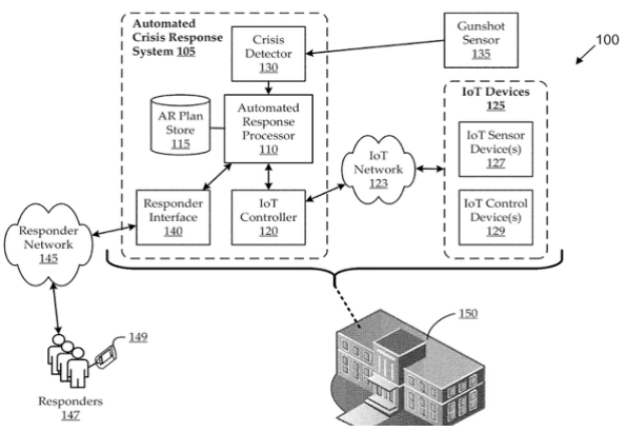
\includegraphics[width=.6\linewidth]{describe-2}
		\caption{US11132889B2 – Automated Crisis Incident Response for Internet of Things Networks}
    	\label{fig:describe-2}
    	\setstretch{2.0}
	\end{figure}
	Execution of the plan may involve automated control of multiple IoT devices installed in and around a facility \autocite{McSchooler2021}. These tools can automate emergency procedures, track personnel, and guide staff through planned response procedures, standardizing crisis response and minimizing confusion during emergencies \autocite{McSchooler2021}. Unfortunately, these solutions often rely on cloud-based communication, assuming personnel have continuous internet access. As a result, while these systems enable coordination under normal conditions, their operational capacity can be impacted when connectivity is compromised.
	
	Solutions to maintaining situational awareness have also included the automated sharing of surveillance video, particularly in 911 dispatch centers \autocite{Drako2020}. During an emergency, the system, as shown in Figure \ref{fig:describe-3}, provides a mechanism that a facility administrator can use to temporarily enable shared access of surveillance video for authorized first responders \autocite{Drako2020}.
	\begin{figure}[H]
		\setstretch{0.8}
		\centering
		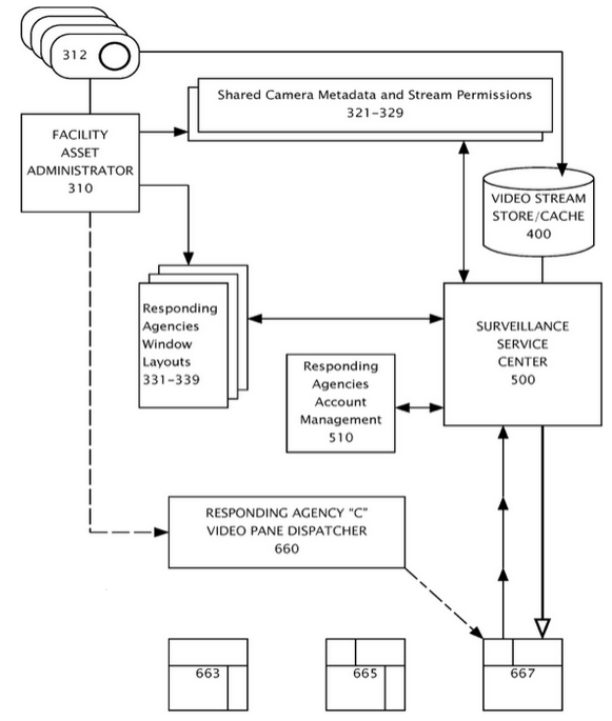
\includegraphics[width=.5\linewidth]{describe-3}
		\caption{US10674116B2 – System and Apparatus for Sharing Private Video Streams with First Responders}
		\label{fig:describe-3}
		\setstretch{2.0}
	\end{figure}
	Set permissions determine what metadata and video streams personnel can access (e.g., camera type, location, motion, facial recognition), allowing responders to securely view this footage via a web or mobile app \autocite{Drako2020}. However, fixed security cameras offer a limited field of view and do not adapt to the changing nature of emergency scenes, especially when upfront infrastructure investments are not prioritized. Additionally, even temporary sharing introduces the risk of unauthorized access or misuse, and web and mobile access for field agents requires network reliability that may fail during crises.
	
	Recent developments in the accuracy and availability of Machine Learning and Large Language Models has led to progress in the aggregation and application of discrete data streams in the IoES space, culminating in crisis management platforms that integrate Large Language Models (LLM) to expand functionality These platforms analyze real-time and historical data to assess impact, delegate resources, and present information and actionable insights using various visualizations \autocite{Ahmad2024}. The integration of these LLMs also enables querying datasets in natural language, reducing the barrier to entry for untrained users \autocite{Ahmad2024}. However, these systems' reliance on high-quality, real-time data collection may lead to latency when field conditions change. Because these systems depend on high-bandwidth data streams and continuous input from infrastructure-based sensors, they cannot operate in degraded infrastructure environments. Stakeholder interviews also revealed that real-time awareness at the on-the-scene level, rather than predictive analytics, is a more pressing gap due to the need for quick resolution of some emergencies.
	All analyses of prior solution attempts show significant advances in data stream fusion, real-time insights, and networked response. However, a consistent limitation across all approaches is reliance on existing infrastructure, including cloud connectivity, fixed sensors, and building-based communication networks.

	\label{Describe Phase - Relevant Math & Science}
	\begin{flushleft}
		\bfseries{Relevant Math \& Science}
	\end{flushleft}
	
	The relative frequency of emergency incidents in the United States has increased rapidly over the past decade \autocite{FBI2024}. As incidents have increased, Law Enforcement response time has decreased, with historical FBI data from 2000-2013 showing an average event duration of ~12 minutes, and recent-year shootings, such as the Perry and Apalachee shootings, falling within the 4-6-minute range \autocite{Tucker2024}.
	
	Additionally, mass shooting events are more likely to occur in workplaces and schools, with historical data showing that they compose 28\% and 22\% of recorded events, respectively \autocite{Rockefeller2025}. Legislative requirements for silent panic button alarms to be installed in public schools, known widely as `Alyssa's Law`, named for the 14-year-old Parkland shooting victim, currently exist; however, they oftentimes are less effective than a simple 911 call, according to the timeline of some of the most recent school shootings \autocite{Tucker2024}. 
	
	Studies of emergency management systems show that a rapid, reliable flow of information directly improves outcomes for emergency victims. A 2020 study found that technologies that enable faster data exchange and real-time updates significantly enhance decision quality, resource deployment, and coordination across agencies \autocite{Kedia2022}. Integrating these data-rich platforms often leads to decision fatigue and cognitive overload for emergency coordinators due to the flood of incoming data. Excessive information can overwhelm responders, leading to slower reaction times and reduced judgment quality, while information overload degrades analytical thinking, causing greater reliance on intuition rather than systematic reasoning \autocite{Roberts2020}.
	
	\label{Describe Phase - Stakeholder Needs}
	\begin{flushleft}
	\bfseries{Stakeholder Needs}
	\end{flushleft}
	
	To identify the project's needs and requirements, interviews were conducted with stakeholders, including business, local, and state-level emergency response coordinators. Across all interviews, stakeholders emphasized the need for a fast, reliable system. The highest-priority areas include direct, delay-free communication between stakeholders, rapid and accurate information distribution, and systems that remain functional even after power or connectivity failures. The importance of a platform that integrates with existing systems and provides simple interfaces for untrained personnel was also highlighted in these interviews, underscoring the need for a human-centered approach to security and decision-making. Additionally, the proposed solution should address gaps in existing response operations, as changes in available personnel or training levels could compromise information accuracy or increase the risk to responders.
	
	
	%/ Generate Phase
	\[
	\begin{array}{cc}
		\mbox{\bfseries{Generate Phase}}
		\label{Generate Phase}
	\end{array}
	\]

	The purpose of the Generate phase is to brainstorm numerous potential solutions that fit the stakeholder needs identified in the previous phase. This brainstorming process was completed as a group and included individual and group brainstorming, mind mapping, and concept sketching. The brainstorming group for this project consisted of three people whose projects were tangentially related, and it was completed during the allotted class time. Each project was given 30 minutes to complete individual and group brainstorming, after which concept sketches were generated based on the proposed ideas. To prevent fixation on initial ideas, a requirement was established that each proposed concept had to be markedly different from the others, ensuring a wide variety of ideas.
	
	After the project concept and key details were explained and the individual and group brainstorming processes were completed, a mind map was created to identify requirement groups and potential solutions, as shown in Figure \ref{fig:generate-1}. The identified categories were based on different needs, including ease of use, speed, multi-modal compatibility, reliability, and accuracy. Potential solutions and blockers to these categories were written on sticky notes for reference during concept sketching.
	
	After completing the mind map, the group moved on to concept sketching, as shown in Figure \ref{fig:generate-2}. These concepts included a mesh-based aerial autonomous system integrated with various sensors to achieve situational awareness, as well as mobile sensors that are independent of building infrastructure.
	
	\begin{figure}[H]
		\setstretch{0.8}
		\centering
		\begin{minipage}{.5\textwidth}
			\centering
			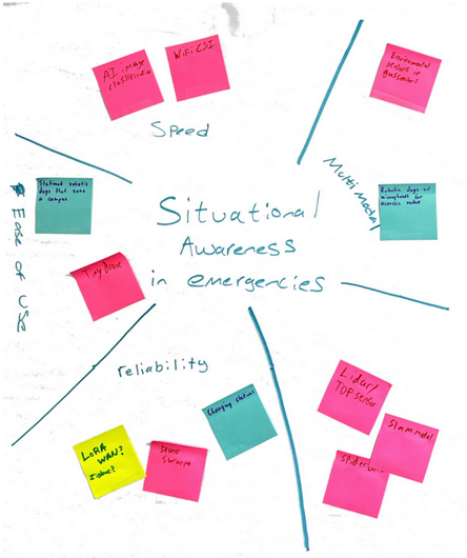
\includegraphics[width=.7\linewidth]{generate-1}
			\caption{Mind Map}
			\label{fig:generate-1}
		\end{minipage}%
		\begin{minipage}{.5\textwidth}
			\centering
			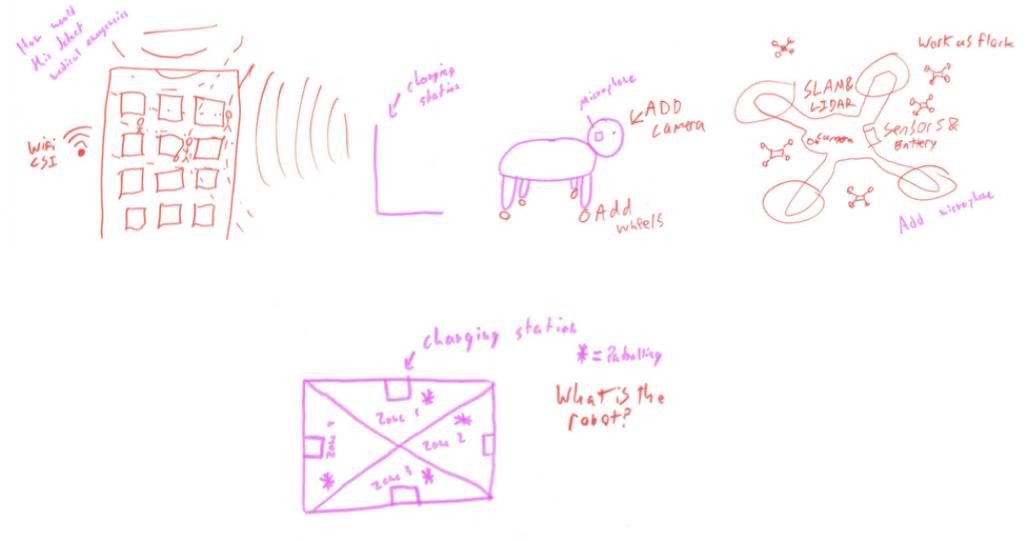
\includegraphics[width=\linewidth]{generate-2}
			\caption{Concept Sketches}
			\label{fig:generate-2}
		\end{minipage}
		\setstretch{2.0}
	\end{figure}

	%/ Select Phase
	\[
	\begin{array}{cc}
		\mbox{\bfseries{Select Phase}}
		\label{Select Phase}
	\end{array}
	\]
	
	The purpose of the Select phase is to evaluate the concepts in the Generate phase, identify their strengths and weaknesses, and select a final design for testing. This phase involves concept analysis using Pugh Charts and risk analysis using a FMEA table. The selected solution should meet all stakeholder needs in a realistic, cost-effective, and technically feasible way.
	
	The design selected to meet these needs is a Bluetooth Low Energy (BLE)-based emergency localization system that enhances situational awareness in distributed environments. This system is comprised of three components: a BLE room-localization network, a mobile interface for stakeholders, and role-based playbooks for users. The implementation of this system will improve staff and first-responder response in emergencies, especially in complex environments such as schools and churches, where defined security roles may be spread thin, and reliance is placed on volunteers and outside collaborators to ensure site safety and perform critical functions. Using room-level BLE beacons and mobile devices, the positions of key personnel and stakeholders can be determined quickly, reducing initial confusion about an emergency's location and enabling the rapid identification of an event's scale and scope. The system is designed from a human-first perspective, reducing cognitive load during emergencies by enabling users to report incidents clearly and guiding them through role-specific playbooks defined by organizational policy. 
	
	To define this design, a series of Pugh charts were created to assess the user interface and communication methods. The Pugh chart allowed ideas to be weighted against themselves and related ideas, depending on how well each idea met a specific stakeholder need and on its relative improvement or regression compared to a datum. The criteria for the Pugh charts were identified from the stakeholder interviews conducted during the Describe phase of this project. They included interoperability with existing systems, coverage area, reliability, latency, duplex communication capability, and the cognitive load required for system use. Additional requirements were identified based on the project's data-sharing requirements, including the ability to handle multimodal data, system security, and scalability. The proposed design, a BLE-based emergency localization system that enhances situational awareness across large or distributed environments, best meets each need identified in the Pugh charts.
	
	The first comparison of stakeholder needs was used to identify the user-facing interface aspect of the system (as shown in Table 1). The selected datum for Table 1 was an existing push-to-talk (PTT) radio system used by numerous security personnel interviewed during the Describe Phase. Improvements to the existing solution used as the datum concept include implementing VoIP-based internet radios to enable clear, duplex communication, a smartphone application, and two personnel-attached devices: a body-worn pack and a voice-activated headset. 
	\begin{figure}[H]
		\begin{minipage}{\textwidth}
			\centering
			\normalfont{Table 1: Pugh Chart \#1 – User Interface Definitio}
			\label{Select Phase - User Interface Pugh Chart}
		\end{minipage}
		\centering
		\setstretch{0.8}
		\begin{adjustbox}{max width=\textwidth}
			\begin{tabular}{l c c c c c}
				\toprule
				\textbf{Criteria} & \textbf{PTT Handheld Radio} & \textbf{VOIP Radio} & \textbf{Smartphone Application} & \textbf{Body Pack} & \textbf{Voice Headset} \\
				\midrule
				Interoperability & 0 & \cellcolor{green!25}1 & \cellcolor{red!25}-1 & \cellcolor{red!25}-1 & \cellcolor{red!25}-1 \\
				Coverage & 0 & \cellcolor{green!25}1 & \cellcolor{green!25}1 & \cellcolor{green!25}1 & \cellcolor{green!25}1 \\
				Reliability & 0 & \cellcolor{red!25}-1 & \cellcolor{red!25}-1 & \cellcolor{red!25}-1 & \cellcolor{red!25}-1 \\
				Latency & 0 & \cellcolor{green!25}1 & \cellcolor{green!25}1 & \cellcolor{green!25}1 & \cellcolor{green!25}1 \\
				Duplex Communication & 0 & \cellcolor{green!25}1 & \cellcolor{green!25}1 & \cellcolor{green!25}1 & \cellcolor{red!25}-1 \\
				Cognitive load & 0 & 0 & \cellcolor{green!25}1 & \cellcolor{red!25}-1 & \cellcolor{red!25}-1 \\
				Deployment & 0 & \cellcolor{red!25}-1 & \cellcolor{green!25}1 & \cellcolor{red!25}-1 & \cellcolor{red!25}-1 \\
				Multimodal Data & 0 & 0 & \cellcolor{green!25}1 & 0 & 0 \\
				Hands-Free Operability & 0 & 0 & 0 & \cellcolor{green!25}1 & \cellcolor{green!25}1 \\
				Security & 0 & \cellcolor{green!25}1 & \cellcolor{green!25}1 & \cellcolor{red!25}-1 & \cellcolor{red!25}-1 \\
				Scalability & 0 & \cellcolor{red!25}-1 & \cellcolor{green!25}1 & \cellcolor{red!25}-1 & \cellcolor{red!25}-1 \\
				\midrule
				\textbf{Total Plus (+)} & & 5 & 8 & 4 & 3 \\
				\textbf{Total Minus (-)} & & -3 & -2 & -6 & -7 \\
				\midrule
				\textbf{Net Score} & & \textbf{+2} & \textbf{+6} & \textbf{-2} & \textbf{-4} \\
				\bottomrule
			\end{tabular}
		\end{adjustbox}
		\setstretch{2.0}
	\end{figure}
	The smartphone application most clearly met each identified need due to its inherent multimodality and widespread ubiquity. Additionally, most users are already familiar with the operation and use of mobile devices, and they are flexible for future development, making them highly adaptable across a variety of environments. The downsides of a mobile application, including potential interoperability issues and reliability concerns, can be mitigated by implementing a plugin-based software stack and mesh-networking features in BLE nodes, along with a long-range radio communication method for dedicated “bridge” nodes. Other solutions, such as the VoIP-based radio, body-worn device, and voice-controlled headset, scored lower than the smartphone application, mainly due to high upfront investment costs, scalability and deployment difficulties, and limited awareness of cognitive burden. For example, by introducing a voice-controlled headset into the day-to-day operations of an organization, not only is the additional overhead of the short-term maintenance and upkeep of the system now an organizational burden, but there is an increased burden on the users themselves as they train to interact with the system in a non-obvious way (e.g., through voice communication). While natural-language systems may be implemented for this use case, the benefits of a smartphone application far outweigh those of a body-worn system. 
	
	\begin{figure}[H]
		\begin{minipage}{\textwidth}
			\centering
			\normalfont{Table 2: Pugh Chart \#2 – Emergency Coordination Definition}
			\label{Select Phase - Emergency Coordination Pugh Chart}
		\end{minipage}
		\centering
		\setstretch{0.8}
		\begin{adjustbox}{max width=\textwidth}
			\begin{tabular}{l c c c c c}
				\toprule
				\textbf{Criteria} & \textbf{Static Guidelines} & \textbf{Rule Based Guidelines} & \textbf{Physical SOS} & \textbf{BLE Room Localizer} & \textbf{Voice Assistant} \\
				\midrule
				Speed of Deployment & 0 & 0 & 0 & 0 & \cellcolor{red!25}-1 \\
				Infrastructure Dependence & 0 & \cellcolor{green!25}1 & \cellcolor{red!25}-1 & \cellcolor{green!25}1 & 0 \\
				Cost & 0 & 0 & \cellcolor{red!25}-1 & \cellcolor{red!25}-1 & \cellcolor{red!25}-1 \\
				Training Burden & 0 & \cellcolor{green!25}1 & 0 & \cellcolor{green!25}1 & \cellcolor{red!25}-1 \\
				Situational Awareness Quality & 0 & 0 & \cellcolor{green!25}1 & \cellcolor{green!25}1 & 0 \\
				Communication Clarity & 0 & \cellcolor{green!25}1 & \cellcolor{red!25}-1 & \cellcolor{green!25}1 & \cellcolor{red!25}-1 \\
				Hands-Free Operability & 0 & \cellcolor{green!25}1 & 0 & \cellcolor{green!25}1 & \cellcolor{green!25}1 \\
				Security & 0 & \cellcolor{green!25}1 & \cellcolor{red!25}-1 & \cellcolor{green!25}1 & 0 \\
				\midrule
				\textbf{Total Plus (+)} & & 5 & 1 & 6 & 1 \\
				\textbf{Total Minus (-)} & & 0 & -4 & -1 & -4 \\
				\midrule
				\textbf{Net Score} & & \textbf{+5} & \textbf{-3} & \textbf{+5} & \textbf{-3} \\
				\bottomrule
			\end{tabular}
		\end{adjustbox}
		\setstretch{2.0}
	\end{figure}
	
	The second comparison of stakeholder needs (as shown in Table 2) used a Pugh chart to identify how IoES technology could be incorporated into the smartphone application (as determined in Table I) to provide actionable insights and data to stakeholders during an event, thereby enhancing their situational awareness. Additional IoES-based data-collection metrics were introduced, including a BLE-based user localization method, a physical emergency alert button in rooms, a real-time, rule-based emergency playbook, and a voice data-collection system. Each option was compared to the datum, an existing solution used by an interviewee that used binders with emergency guidelines in each room on campus. Each concept was evaluated against stakeholder criteria, including training burden, increase in situational awareness, level of infrastructure independence, and clarity of communication under stress. Of the identified concepts, two additions to the smartphone application were prioritized: the dynamic rule-based emergency guideline system and the BLE room localization system.
	
	After a specific plan was selected, Failure Mode Effects Analysis (as shown in Appendix I) was conducted to identify potential failure modes in the proposed solution. Several potential failure areas were identified, including battery depletion in BLE nodes, corrupted beacon firmware, signal quality issues, and reliance on volunteer devices. Issues related to battery depletion, corrupted firmware, and signal quality can be mitigated by incorporating additional telemetry during system operation and by collecting aggregated mesh-network health data. These are technology- and implementation-specific issues that fall outside the scope of the current phase and will be addressed during the Embody phase of the project. Other issues have more critical effects, such as relying on the mobile app to estimate the responder’s current room, which could lead to misrepresentation of the current location or the system failing altogether. To mitigate the effects of this occurrence, dedicated response devices should be available in each response zone for use during emergencies, and the project scope should be expanded to include less infrastructure-dependent communication strategies, such as using the mesh network itself for low-cost communication updates.
	
	The identified solution, a system comprising Bluetooth-based room localization and a smartphone application, directly addresses the limitations of infrastructure-dependent emergency platforms identified in the research conducted during the Describe phase. Unlike Integrated Emergency Data Platforms and fixed IoT networks that rely on internet access and power stability, this system operates independently of building infrastructure and remains functional even in degraded environments. BLE beacons provide accurate room-level location without GPS or Wi-Fi, and the smartphone application can be deployed anywhere in the field alongside volunteers. The smartphone- and dedicated-device-based interface helps reduce cognitive overload by providing volunteers with structured interactions and organization-defined playbooks, rather than complex, proprietary interfaces and excessive data. By taking this approach, stakeholder priorities for mobile, resilient, and easy-to-use solutions are met, and situational awareness is facilitated for both trained responders and untrained volunteers during time-sensitive emergencies.
	
	%/ Embody Phase
	\[
	\begin{array}{cc}
		\mbox{\bfseries{Embody Phase}}
		\label{Embody Phase}
	\end{array}
	\]
	
    The purpose of the Embody phase is to design, assemble, and test the concept selected in the select phase, identify the concept's strengths and weaknesses through testing, and finalize a design that meets all stakeholder needs, as determined through the iterative testing completed in this phase. Two initial prototypes were assembled to validate the core functionality of the system's individual components before integrating them into a final design. The prototype includes four main components: a 3.7V 1200mAh lithium-ion polymer (LiPo) battery, a Power over Ethernet (PoE) to 5-volt DC converter, an nRF52 System-on-Chip (SoC) developer module, and a LoRa (Low Power Wide Range) radio. A React Native application running on a mobile device was also developed with the  prototype to test communication between the user interface and the mesh nodes. Each component was selected to test the system's requirements as defined by the stakeholder needs, and the following tests were used to evaluate the capabilities of the proposed solution. 
	
	The first test of the prototype system was to determine its battery life of the system under simulated degraded (loss of power) infrastructure conditions, to ensure that stakeholders' need for infrastructure independence and reliability in degraded environments is met. The test was conducted on two assembled nodes (short- and long-range) with varying levels of simulated mesh activity to model how communication strain could affect the system. Tests were conducted with and without the LoRA radios to determine how the increased transmission power required would affect the battery's lifespan. To conduct this test, the battery was charged using the nRF52 board's built-in battery charger, then all external power was removed from the system. The battery voltage at the beginning of the test was recorded, then a BLE beacon was broadcast every 5, 15, and 30 seconds for an hour, and the ending voltage was recorded.

	\begin{figure}[H]
		\begin{minipage}{\textwidth}
			\centering
			\normalfont{Table 3: Test \#1 - Battery Life}
			\label{Test 1 - Battery Life}
		\end{minipage}
		\centering
		\setstretch{0.8}
		\scriptsize
		\begin{tabular}{>{\raggedright\arraybackslash}p{3.5cm} >{\centering\arraybackslash}p{1.5cm} >{\centering\arraybackslash}p{2cm} >{\centering\arraybackslash}p{2cm} >{\centering\arraybackslash}p{2cm} >{\centering\arraybackslash}p{2cm}}
			\toprule
			\textbf{System Description} & \textbf{Interval (s)} & \textbf{Starting Voltage} & 	\textbf{Ending Voltage} & \textbf{Elapsed Time} & \textbf{Est. Total Runtime} \\
			\midrule
			Short Range Node [BLE Only] & 5 & 3.842 V & 3.806 V & 1 hr & $\sim$115 hr \\
			Short Range Node [BLE Only] & 15 & 3.817 V & 3.804 V & 1 hr & $\sim$335 hr \\
			Short Range Node [BLE Only] & 30 & 3.863 V & 3.857 V & 1 hr & $\sim$950 hr \\
			\midrule
			Long Range Node [BLE + LoRA] & 5 & 3.826 V & 3.689 V & 1 hr & $\sim$24 hr \\
			Long Range Node [BLE + LoRA] & 15 & 3.851 V & 3.800 V & 1 hr & $\sim$80 hr \\
			Long Range Node [BLE + LoRA] & 30 & 3.808 V & 3.789 V & 1 hr & $\sim$225 hr \\
		\end{tabular}
		\begin{tabular}{>{\raggedright\arraybackslash}p{9cm} >{\centering\arraybackslash}p{2.5cm} >{\centering\arraybackslash}p{2.5cm}}
			\toprule
			\textbf{Operation} & \textbf{Est. Current Draw} & \textbf{Duration} \\
			\midrule
			System On & 1.9 $\mu$A &\\
			BLE Advertising & 5.3 mA & $\sim$4.5 ms/event \\
			BLE Scan Window & 5.6 mA & Variable \\
			BLE RX & 4.6 mA & $\sim$1.2 ms/packet \\
			CPU & 3.7 mA & Variable \\
			\midrule
			LoRA Sleep & 0.2 $\mu$A & \\
			LoRA TX  & 120 mA & $\sim$50 ms/packet \\
			LoRA RX Window & 10.3 mA & $\sim$25 ms \\
			\midrule
			\textbf{Totals: Short Range Node} & & \\
			\quad 5s Interval (avg) & $\sim$4.27 mA &  \\
			\quad 15s Interval (avg) & $\sim$1.48 mA &  \\
			\quad 30s Interval (avg) & $\sim$0.53 mA &  \\
			\midrule
			\textbf{Totals: Long Range Node} & & \\
			\quad 5s Interval (avg) & $\sim$17.24 mA &  \\
			\quad 15s Interval (avg) & $\sim$6.10 mA &  \\
			\quad 30s Interval (avg) & $\sim$2.19 mA &  \\
			\bottomrule
		\end{tabular}
		\setstretch{2.0}
	\end{figure}
	
	As shown in Table 3, the data collected from each iteration of the test shows no concern for infrastructure independence in emergency situations, with a mean activation time of 467 hours for short-range nodes and 110 hours for long-range nodes. Research on emergency event lengths and timelines indicates that emergency events requiring the proposed system would be short, lasting minutes rather than hours, meaning that this system has enough battery capacity to fulfill the stakeholders requirements for an infrastructure-independent solution that can operate in times of crisis. 
	
	The second test of the system was to determine the accuracy of BLE localization in the mobile app. The test was conducted by changing both the nRF52 BLE output power and the mobile device's distance from the node, recording the change in Received Signal Strength Indicator (RSSI) at each setting and the output distance from the application. This establishes a signal profile using the log-distance path loss model, improving the localization algorithm's accuracy in determining a device's position within a building. The log-distance path loss model is a representation of how signal strength shifts over changes in distance, according to: 
	\begin{equation}
		RSSI(d) = RSSI(d_0) - 10 \cdot n \cdot \log_{10}\!\left(\frac{d}{d_0}\right)
	\end{equation}
	\noindent
	where $d$ is the distance to the beacon, $d_0$ is the reference distance (1 meter), $RSSI(d_0)$ is the signal strength at the reference distance, and $n$ is the path loss exponent. By establishing $n$ by measuring the RSSI at a 1 meter distance for each output level and changing $d$, the mobile device can accurately calculate distance across all power levels.
	
	To conduct this test, the user device was moved within a room at distances of 1, 3, and 5 meters from the node, while the RSSI strength was recorded at each position across the four power levels shown using the log-distance path loss model.
	
	\begin{figure}[H]
		\begin{minipage}{\textwidth}
			\centering
			\normalfont{Table 4: Test \#2 - BLE Localization}
			\label{Test 2 - BLE Localization}
		\end{minipage}
		\centering
		\setstretch{0.8}
		\scriptsize
		\begin{tabular}{>{\centering\arraybackslash}p{3.5cm} >{\centering\arraybackslash}p{3.5cm} >{\centering\arraybackslash}p{3.5cm} >{\centering\arraybackslash}p{3.5cm}}
			\toprule
			\textbf{Output Power} & \textbf{Real Distance from Node} & \textbf{Recorded RSSI} & \textbf{Calculated Distance} \\
			\midrule
			& 1 Meter & -42 dBm & 1 m \\
			+4 dBm & 3 Meters & -52 dBm & 3 m \\
			& 5 Meters & -59 dBm & 5 m \\
			\midrule
			& 1 Meter & -44 dBm & 1 m \\
			0 dBm & 3 Meters & -56 dBm & 3 m \\
			& 5 Meters & -63 dBm & 5 m \\
			\midrule
			& 1 Meter & -50 dBm & 1 m \\
			-4 dBm & 3 Meters & -60 dBm & 3 m \\
			& 5 Meters & -67 dBm & 6 m \\
			\midrule
			& 1 Meter & -52 dBm & 1 m \\
			-8 dBm & 3 Meters & -64 dBm & 3 m \\
			& 5 Meters & -72 dBm & 6 m \\
			\bottomrule
		\end{tabular}
		\doublespacing
	\end{figure}
	As shown in Table 4, data collected from each test iteration shows a direct correlation between real distance and the calculated distance from the node as RSSI varies, confirming the stakeholder device's ability to determine its room-level position relative to the node within a building, regardless of beacon transmission power.
	
	The third test of the system was to determine the maximum effective range of the LoRa radios indoors, to ensure that mesh-based communication between long-range bridge nodes is possible. The test was conducted to determine whether the LoRa radio, operating at 900 MHz with an antenna not typically designed for indoor communications, can maintain acceptable data rates across the distances required by a distributed campus. To do this test, 50 packets were sent between two LoRa nodes at measured distances of 10, 25, and 50 feet on a single floor, as well as between the floors of a multi-story building. RSSI (signal-to-noise ratio) and packet rate were recorded at each position. The tests were conducted both in a traditional multi-story building and in portable buildings to determine the impact of differences in building material signal characteristics.
	
	\begin{figure}[H]
		\begin{minipage}{\textwidth}
			\centering
			\normalfont{Table 5: Test \#3 - LoRa Communication}
			\label{Test 3 - LoRa Communication}
		\end{minipage}
		\centering
		\setstretch{0.8}
		\scriptsize
		\begin{tabular}{>{\raggedright\arraybackslash}p{2.2cm} >{\centering\arraybackslash}p{1.4cm} >{\centering\arraybackslash}p{1.4cm} >{\centering\arraybackslash}p{1.4cm} >{\centering\arraybackslash}p{1.4cm} >{\centering\arraybackslash}p{1.4cm} >{\centering\arraybackslash}p{1.4cm}}
			\toprule
			\textbf{Location} & \textbf{Floor} & \textbf{Distance (ft)} & \textbf{RSSI (dBm)} & \textbf{SNR (dB)} & \textbf{Packets Sent} & \textbf{Success Rate (\%)} \\
			\midrule
			 & 0 & 10 & -67 & 9.2 & 50 & 100 \\
			 & 0 & 25 & -78 & 6.8 & 50 & 100 \\
			Main Building & 0 & 50 & -91 & 3.1 & 50 & 90 \\
			 & 1 &  & -96 & 1.3 & 50 & 82 \\
			 & 2 &  & -103 & -2.1 & 50 & 64 \\
			\midrule
			 &  & 10 & -74 & 6.4 & 50 & 100 \\
			Portables &  & 25 & -89 & 2.7 & 50 & 86 \\
			 &  & 50 & -101 & -1.4 & 50 & 68 \\
			\bottomrule
		\end{tabular}
		\setstretch{2.0}
	\end{figure}
	As shown in Table 5, the data collected from each test shows that single floor transmission at short distances had a 100\% success rate in the main building, while signal degradation increased with distance, floor separation, and more metal dense building construction. The portable buildings at 50 feet showed a 68\% success rate compared to 90\% at the same distance in the main building. These results better inform the recommended density of long-range bridge nodes per floor or per cluster of distributed buildings to one node, depending on the building materials and the surrounding signal characteristics of the environment. This fact will help inform the cost breakdown further on.
	
	The fourth test of the system was to verify that communication between the mobile application and the mesh network of nodes is working. The test was conducted by triggering an emergency event from a user device running the application and checking to ensure that the event was successfully transmitted through the network and that the playbook system assigned role-based tasks to a connected user. To conduct this test, an emergency event was triggered from the application menu, and the backend data logs were recorded to verify that both the event creation and task assignment payloads were transmitted and received correctly.
	\begin{figure}[H]
		\setstretch{0.8}
		\centering
		\begin{minipage}{.4\textwidth}
			\centering
			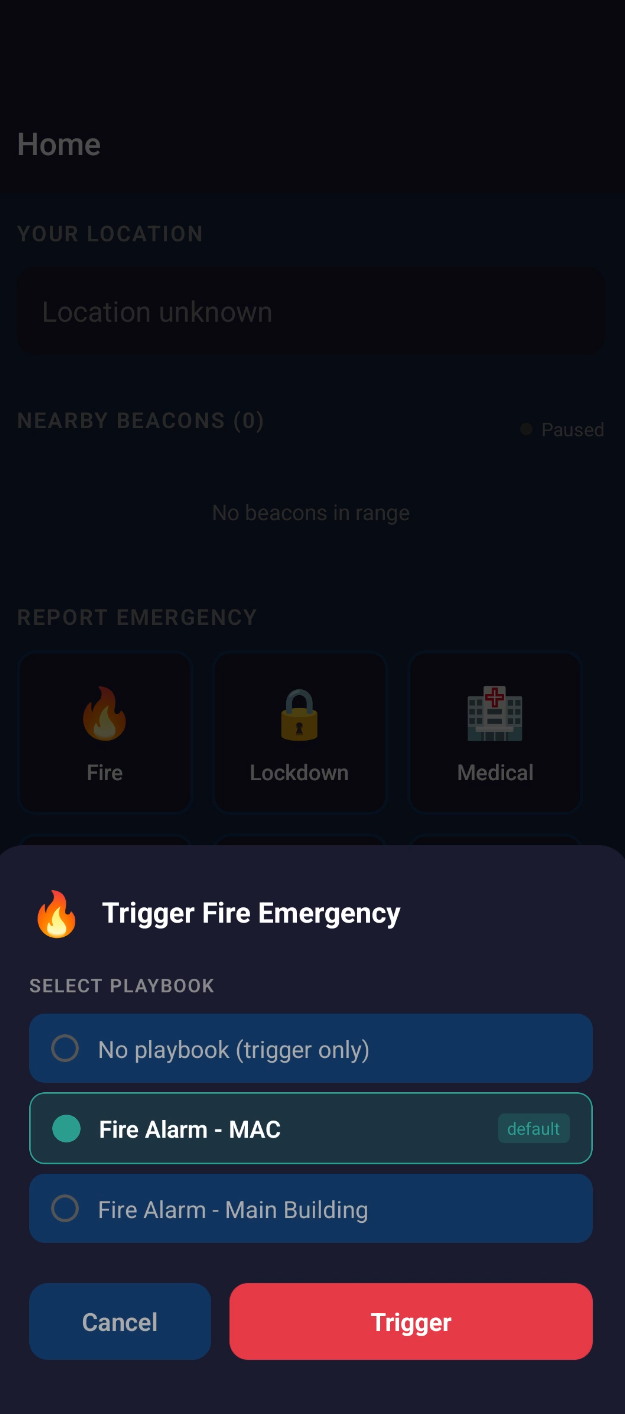
\includegraphics[width=.7\linewidth]{embody-2}
			\caption{Application Trigger Menu}
			\label{fig:embody-2}
		\end{minipage}
		\begin{minipage}{.4\textwidth}
			\centering
			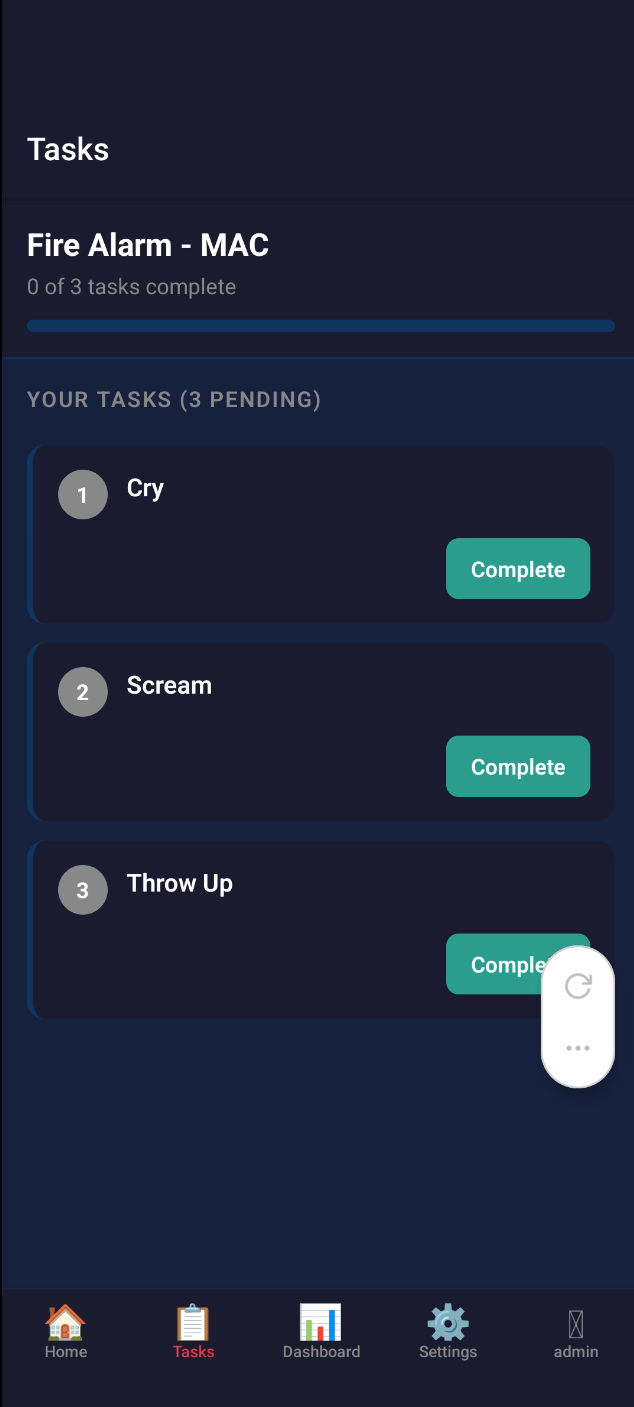
\includegraphics[width=.7\linewidth]{embody-3}
			\caption{Application Event Menu}
			\label{fig:embody-3}
		\end{minipage}
	\end{figure}
	This test confirmed that the system can receive an emergency activation from a stakeholder's device, distribute the alert across both the internet, and the local mesh network, and assign tasks to users based on their assigned roles, as shown in Figures \ref{fig:embody-2} and \ref{fig:embody-3}.
	
	%/ Final Prototype
	\label{Final Prototype}
	\begin{flushleft}
		\bfseries{Final Prototype}
	\end{flushleft}
	
	The final device (shown in Figure 9 \& 10) has two configurations that enable room-level localization and mesh-based emergency communication: a short-range and a long-range node. Each node is built around the nRF52 System-on-Chip (SoC) running the Zephyr Real-Time Operating System and broadcasts BLE advertisements that enable room-level localization on stakeholders' mobile devices. Each node is powered through Power over Ethernet (PoE) during normal operation and can fall back onto an onboard 3.7V 1200mAh Lithium-Ion Polymer (LiPo) battery during periods of infrastructure degradation. The nRF52 is a low-power SoC designed for IoT applications that includes a 32-bit ARM processor and a built-in 2.4 GHz radio that supports BLE. Compared to an ESP32 or Arduino microcontroller, the nRF52 series of SoCs provides the technical capabilities and flexibility required for IoT applications that interact with other devices, such as other nodes in the system or stakeholders' mobile devices. This SoC was additionally selected for its integration with the Zephyr Real Time Operating System (RTOS) for embedded devices, enabling extreme low-power operation while still incorporating a complex Bluetooth Low Energy stack that matches the technical complexity of this system. The Zephyr RTOS was selected for development due to its enhanced implementation of the Serial Port Interface protocol, which was required for interaction with the LoRA Radio.
	
	\begin{figure}[H]
		\setstretch{0.8}
		\centering
		\begin{minipage}{\textwidth}
			\centering
			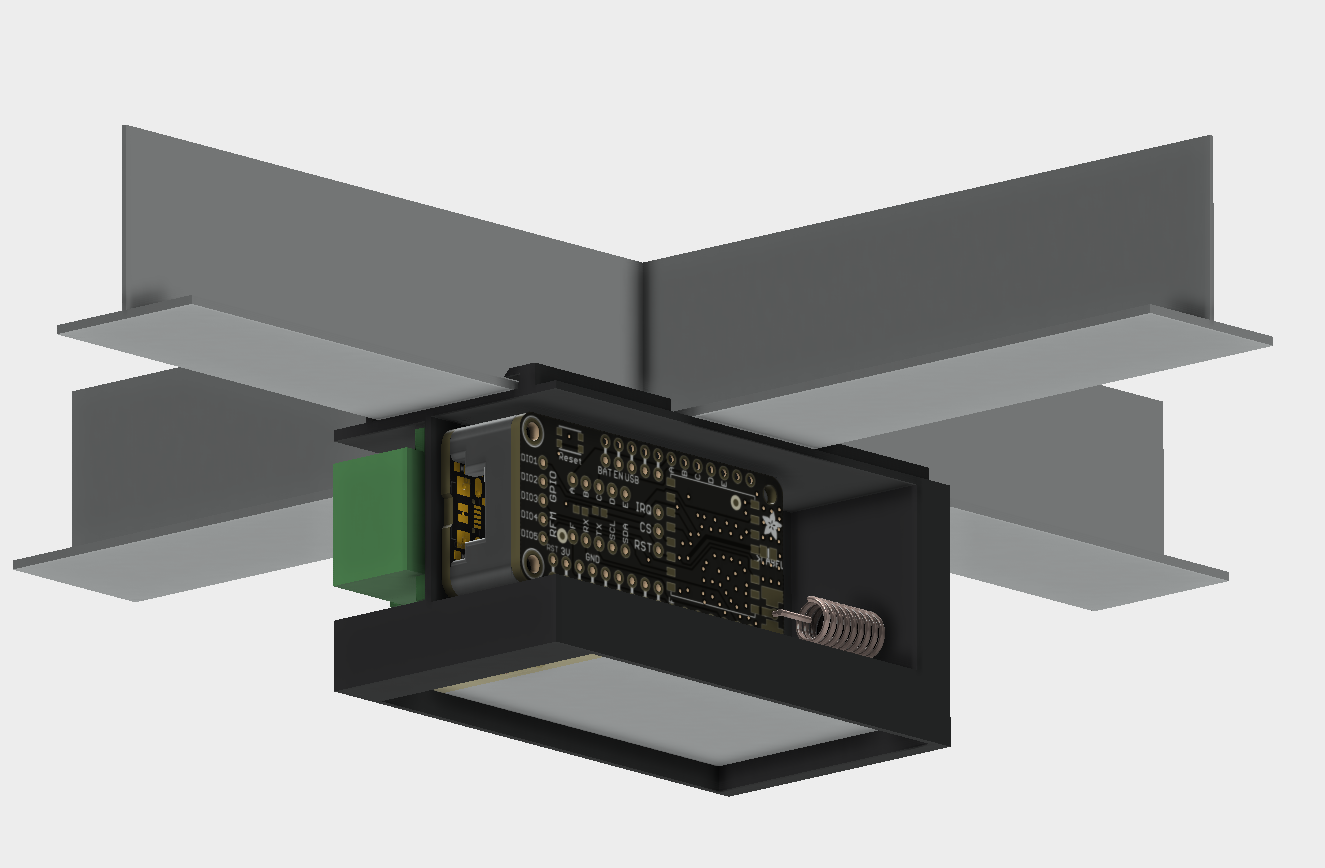
\includegraphics[width=.6\linewidth]{embody-1}
			\caption{CAD Render of the Final Prototype}
			\label{fig:embody-1}
		\end{minipage}
		\setstretch{2.0}
	\end{figure}
	\begin{figure}[H]
		\setstretch{0.8}
		\centering
		\begin{minipage}{.6\textwidth}
			\centering
			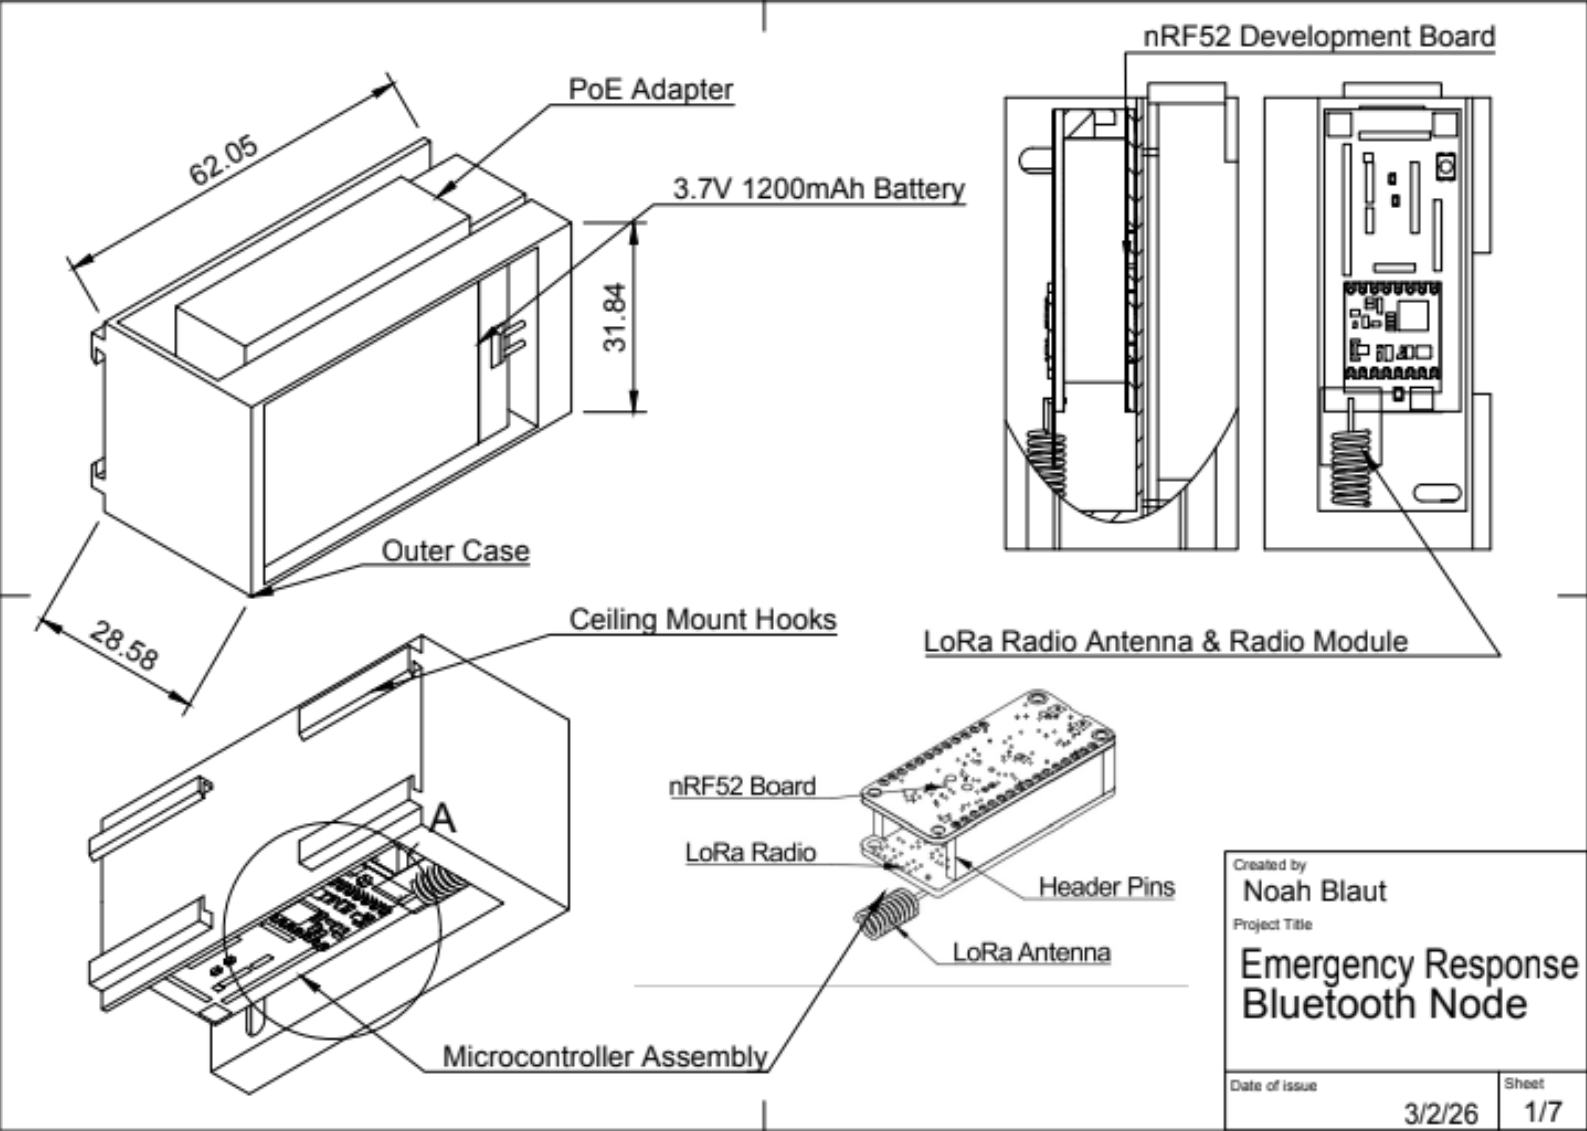
\includegraphics[width=\linewidth]{embody-1b}
			\caption{Technical Sketch of the Final Prototype}
			\label{fig:embody-1b}
		\end{minipage}
		\setstretch{2.0}
	\end{figure}
	
	Unlike short-range nodes, long-range nodes include a LoRa radio operating in the 900 MHz band to transfer data over greater distances and across distributed buildings, where BLE communication alone is insufficient. The LoRA radio was selected for its long-distance intra-mesh communication capabilities, as it provides much more stable data transfer over longer distances between nodes than Bluetooth Low Energy, enabling true infrastructure-independent communication during an emergency event.
	
	The React Native application serves as the interface for stakeholders' interaction with the system. The application receives BLE signals and can use the data within to calculate the user's current room. The mobile application then displays this location on a facility floor plan during an emergency event, allows users to trigger emergency alerts that send an online alert, and spreads the alert throughout the mesh network for redundancy. Upon the activation of an emergency alert, the rule-based playbook system guides each stakeholder through a defined sequence of role-specific tasks set by organizational policy. The mobile application includes different access levels, as set by organizational policy, so that each stakeholder has access to the appropriate amount of information for the role they have been assigned (admin, security, teacher, volunteer, etc.).
	
	%/ Design Defense
	\[
	\begin{array}{cc}
		\mbox{\bfseries{Design Defense}}
		\label{Design Defense}
	\end{array}
	\]
	
	\label{Design Defense - One}
	\begin{flushleft}
		\bfseries{Design Defense \#1: The increased reliance on a user device during an emergency situation may hinder emergency communication.}
	\end{flushleft}
	
	
	One counterargument to the proposed solution is about the reliance on stakeholders' personal mobile devices as the  interface with the system. Some may say that depending on personal devices introduces risk, as users may have their phones powered off, silenced, or packed away. In an emergency situation where seconds matter, the failure a small number of stakeholder devices could hinder the ability of the system to maintain accurate situational awareness, which stakeholders identified as a critical requirement.
	
	However, the decision to use a mobile application as the user interface was made as it provides better latency, reduced cognitive load, the ability for multimodal data handling, and increases in security. The commonality of smartphones reduces the need for additional hardware and user training, which addresses the issue this project tried to solve, that high installation costs and overhead dissuade organizations from investing in life-saving technology. Requiring an organization to purchase and distribute dedicated hardware to every single stakeholder would add cost and complexity barriers while increasing the training burden and long-term maintenance that stakeholders wanted to avoid in interviews. FMEA table analysis also showed "volunteer fails to carry device" as a failure and identified countermeasures, including a select few number of dedicated response devices stationed in critical zones for use during emergencies, and organizational standards that set policy for device usage.
	
	\label{Design Defense - Two}
	\begin{flushleft}
		\bfseries{Design Defense \#2: The proposed solution is not truly "infrastructure free," as it relies on PoE being available within the building that the system is deployed within.}
	\end{flushleft}
	
	Another counterargument to the proposed solution is that this system is not truly "infrastructure-free," as it relies on PoE availability during normal day-to-day operations. As PoE is part of building infrastructure, powering things like Wi-Fi routers and VoIP phones within a campus, the system relies on that infrastructure to operate on a day-to-day basis.
	
	
	However, creating an ultra-low-power microcontroller using off-the-shelf components is difficult, as manufacturers such as Adafruit typically do not prioritize power efficiency as their primary design goal when laying out the design of their Printed Circut Boards (PCBs). For this prototype to be fully "infrastructure independent," a custom PCB would need to be designed to implement more of the ultra-low-power features that the nRF52 provides, which the manufacturer of the current prototype board did not implement. However, PoE provides a suitable alternative for large, distributed campuses that already have a wireless networking strategy in place, as this system can easily hook into that same infrastructure on a day-to-day basis while still being able to operate independently during emergencies by employing the use of the built-in backup battery.
	
	%/ Future Considerations
	\[
	\begin{array}{cc}
		\mbox{\bfseries{Future Considerations}}
		\label{Future Considerations}
	\end{array}
	\]
	
	The solution to a wide variety of issues that are present in this prototype would be to create and manufacture a fully custom PCB that incorporates each electronic component onto one defined package. This would reduce organizational challenges such as the cost of the system, as each component would be custom picked for the one goal of enabling this project and profit margins would be thinner than purchasing many Commercial Off the Shelf (CoTS) products, while also creating improvements in things such as power efficiency and packaging, improving the overall functionality of the product as well. 
	
	While custom PCB manufacturing was explored as a potential possibility, limitations on single-board ordering, component availability, as well as overall design constraints and knowledge gaps prevented it from being viable for this project, but would be the logical next iterative step in the design process of this product. Additionally, testing the node communication over a wider variety of building architectures and mobile devices would better inform the localization accuracy of the system and aid in estimating a more exact node-to-room ratio depending on specific building characteristics. 
	
	%/ Conclusion
	\[
	\begin{array}{cc}
		\mbox{\bfseries{Conclusion}}
		\label{Conclusions}
	\end{array}
	\]
	The frequency of emergency incidents has increased awareness about how organizations maintain situational awareness and coordinate response during rapidly evolving events. This emergency localization system provides low-cost room-level positioning, mesh-based communication, and role-specific playbooks that operate independently of building infrastructure, solving issues identified with existing systems. Through  testing, the proposed system has shown the ability for extended operation during infrastructure degradation, accurate room-level positioning, reliable distance communication across distributed buildings, and successful emergency coordination and communication capabilities. By lowering the barrier for implementation, this system allows schools, churches, and other organizations to implement life-saving emergency communication technology without any overhead that could potentially dissuade investment.
	
	\pagebreak
	%/ Appendix [X]:
	\[
	\begin{array}{cc}
		\mbox{\bfseries{Appendix 1: Failure Mode Effects Analysis Table}}
	\end{array}
	\]
		\begin{figure}[H]
		\begin{minipage}{\textwidth}
			\centering
		\end{minipage}
		\centering
		\setstretch{1.5}
		\scriptsize
		\begin{tabular}{>{\raggedright\arraybackslash}p{2.4cm} >{\raggedright\arraybackslash}p{1.3cm} >{\raggedright\arraybackslash}p{2.2cm} c >{\raggedright\arraybackslash}p{1.8cm} c >{\raggedright\arraybackslash}p{2.4cm}}
			\toprule
			\textbf{Component/ Function} & \textbf{Failure Mode} & \textbf{Effects} & \textbf{Severity} & \textbf{Causes} & \textbf{Probability} & \textbf{Actions} \\
			\midrule
			BLE Room Beacon - Transmit signal & No function & Beacon stops, room undetectable & 3 & Overuse, lack of maintenance & 5 & Long-life batteries; test schedule; battery indicator; PoE lines \\
			\midrule
			BLE Room Beacon - Broadcast ID & Intermittent & Can't map signal to room, location errors & 3 & Corrupted firmware, ID corrupted/reset & 1 & Lock firmware, verify ID in app; label devices \\
			\midrule
			BLE Room Beacon - Signal strength & Intermittent & Signal weak/inconsistent, wrong room & 1 & Placed behind obstruction or wrong spot & 2 & Standard positions; test signal at install \\
			\midrule
			Mobile App - Detect beacon & Degraded & No location update & 1 & Settings/config; BLE fails/disabled & 3 & On-prem devices; startup check; alert if disabled \\
			\midrule
			Mobile App - Estimate room & Degraded & Wrong location, misdirected response & 5 & Incorrect RSSI/wrong room & 2 & Smoothing/filtering; confidence score; manual override \\
			\midrule
			Mobile App - Report location & No function & Commander never sees update & 5 & Data not transmitted & 1 & Retry logic; log fails; queue updates \\
			\midrule
			Beacon Network - Room coverage & No function & Blind spots, untrackable rooms & 4 & Not enough beacons/gaps & 3 & Floor-plan guide; walkthrough verify \\
			\midrule
			Volunteer - Carry device & No function & Volunteer untrackable & 2 & Phone in bag or off & \{x\} & Train protocol; reminders; auto-start \\
			\bottomrule
		\end{tabular}
		\setstretch{2.0}
	\end{figure}
	
		\pagebreak
	%/ Appendix [X]:
	\[
	\begin{array}{cc}
		\mbox{\bfseries{Appendix 2: Code Repository for Project}}
	\end{array}
	\]
	\begin{center}
		Github Repository:
		\quad
		\qrcode[height=1in]{https://github.com/UntitledMoose/EngineeringSeniorThesis}
		\hyperbaseurl{https://github.com/UntitledMoose/EngineeringSeniorThesis}
	\end{center}
	\begin{center}
		https://github.com/UntitledMoose/EngineeringSeniorThesis
	\end{center}
	%\lstinputlisting[language=C,style=myStyle]{/home/untitledmoose/Projects/EngineeringSeniorThesis/hardware/firmware/application/app/src/main.c}
	
	%/ Works Cited
	\pagebreak
	\[
	\begin{array}{cc}
		\mbox{Works Cited}
	\end{array}
	\]
	\vspace{-1cm}
	\printbibliography
	
\end{document}
